\documentclass[journal]{IEEEtran}
\usepackage[utf8]{inputenc}
%\usepackage{minted}
\usepackage{booktabs}
\usepackage{color}
\usepackage{commath}
\usepackage{tikz}
\usepackage[official]{eurosym}
\usepackage{fontawesome}
\usepackage{breqn}
\usepackage{float}

\usepackage[binary-units=true]{siunitx}

%\newcommand{\py}[1]{\mintinline{python}{#1}}

\title{Artificial Intelligence (\texttt{LINGI2261}) \\ Assignment 2 --- Group 13}
\author{Martin Braquet, Gilles Peiffer}

\begin{document}

\maketitle

\section{A* versus uniform-cost search}

\subsection{A consistent and admissible heuristics}

A valid heuristics for this problem is the Manhattan distance between the two symbols positions, which is the minimum distance between them expressed in number of tiles.

It is consistent for an unweighted grid since at each move, the traveller can at most decrease by one its remaining cost to the goal while this heuristics is also decreased by one. Formally, for every node $N$ and each successor $P$ of $N$, the consistency states that the estimated cost of reaching the goal from $N$ is no greater than the step cost of getting to $P$ plus the estimated cost of reaching the goal from $P$:
\[
 h(N) \le c(N,P) + h(P)
\]
In our case, let us define $N = (x_N, y_N)$ by its coordinates on the 2D grid. In the same way, we define $P = (x_P, y_P)$ and the goal $G = (x_G, y_G)$. The inequality is thus rewritten as
\[
 \abs{x_N - x_G} + \abs{y_N - y_G} \le 1 + \abs{x_P - x_G} + \abs{y_P - y_G}
\]
where $c(N,P) = 1$ since $P$ is the successor of $N$ and the grid is unweighted. Using the trangle inequality, one can rewrite $\abs{x_N - x_G} + \abs{y_N - y_G}$ as 
\begin{align*}
   & \abs{x_N - x_P + x_P - x_G} + \abs{y_N - x_P + x_P - y_G} \\
  \le & \abs{x_N - x_P} + \abs{x_P - x_G} + \abs{y_N - x_P} + \abs{x_P - y_G} \\
  \le & 1 + \abs{x_P - x_G} + \abs{x_P - y_G}
\end{align*}
where $\abs{x_N - x_P} + \abs{x_N - y_P} = 1$ since the traveller moves by one title horizontally or vertically. It has thus been proven that this heuristics is consistent.

If an heuristics is consistent, it is also admissible.
The Manhattan distance is thus also always lower than or equal to the real number of moves to the goal. Formally, $h(h)$ is admissible if, $\forall n$, $h(n) \le C^*$ where $C^*$ is the lowest path cost among all solutions. Since each action can move only one tile, performing an action can at most reduce $h$ by one. Since the goal can be reached in $C^*$ actions, we thus have $h(n) - C^* \le h(G) = 0$. Therefore, we have $h(n) \le C^*$ forall $n$, and $h$ is admissible.

\subsection{Uniform-cost graph search}

The visited nodes (in light gray) for the uniform-cost graph search are depicted in Figure \ref{fig:maze1}, the number in each tile decribes the order of the visited states. The uniform-cost search finds the solution when it reaches the 25th state.

\begin{figure}[H]
 \centering
 \begin{tikzpicture}
    [
        box/.style={rectangle,draw=black,thick, minimum size=1cm},
    ]

    \foreach \x in {1,...,7}{
        \foreach \y in {1,...,7}
            \node[box] at (\x,\y){};
    }

    \node[box,fill=black] at (6,7){};
    \node[box,fill=black] at (6,6){};
    \node[box,fill=black] at (5,6){};
    \node[box,fill=black] at (4,5){};
    \node[box,fill=black] at (3,5){};
    \node[box,fill=black] at (2,5){};
    \node[box,fill=black] at (3,4){};
    \node[box,fill=black] at (3,3){};
    \node[box,fill=black] at (3,2){};
    \node[box,fill=black] at (2,2){};
    \node[box,fill=black] at (7,4){};
    \node[box,fill=black] at (7,3){};
    \node[box,fill=black] at (7,2){};
    
    \node[box,fill=lightgray] at (5,7){};
    \node[box,fill=lightgray] at (4,7){1};
    \node[box,fill=lightgray] at (3,7){2};
    \node[box,fill=lightgray] at (4,6){3};
    \node[box,fill=lightgray] at (2,7){4};
    \node[box,fill=lightgray] at (3,6){5};
    \node[box,fill=lightgray] at (1,7){6};
    \node[box,fill=lightgray] at (2,6){7};
    \node[box,fill=lightgray] at (1,6){8};
    \node[box,fill=lightgray] at (1,5){9};
    \node[box,fill=lightgray] at (1,4){10};
    \node[box,fill=lightgray] at (1,3){11};
    \node[box,fill=lightgray] at (2,4){12};
    \node[box,fill=lightgray] at (1,2){13};
    \node[box,fill=lightgray] at (2,3){14};
    \node[box,fill=lightgray] at (1,1){15};
    \node[box,fill=lightgray] at (2,1){16};
    \node[box,fill=lightgray] at (3,1){17};
    \node[box,fill=lightgray] at (4,1){18};
    \node[box,fill=lightgray] at (4,2){19};
    \node[box,fill=lightgray] at (5,1){20};
    \node[box,fill=lightgray] at (4,3){21};
    \node[box,fill=lightgray] at (5,2){22};
    \node[box,fill=lightgray] at (6,1){23};
    \node[box,fill=lightgray] at (4,4){};
    
    \node[box] at (5,7){\faMale};
    \node[box] at (4,4){\euro{}};

 \end{tikzpicture}
 \caption{Visited nodes (in light gray) for the uniform-cost graph search}
 \label{fig:maze1}
\end{figure}

\subsection{A* graph search}

The visited nodes (in light gray) for the A* graph search are depicted in Figure \ref{fig:maze2}. A* finds the solution when it reaches the 21th state.

\begin{figure}[H]
 \centering
 \begin{tikzpicture}
    [
        box/.style={rectangle,draw=black,thick, minimum size=1cm},
    ]

    \foreach \x in {1,...,7}{
        \foreach \y in {1,...,7}
            \node[box] at (\x,\y){};
    }

    \node[box,fill=black] at (6,7){};
    \node[box,fill=black] at (6,6){};
    \node[box,fill=black] at (5,6){};
    \node[box,fill=black] at (4,5){};
    \node[box,fill=black] at (3,5){};
    \node[box,fill=black] at (2,5){};
    \node[box,fill=black] at (3,4){};
    \node[box,fill=black] at (3,3){};
    \node[box,fill=black] at (3,2){};
    \node[box,fill=black] at (2,2){};
    \node[box,fill=black] at (7,4){};
    \node[box,fill=black] at (7,3){};
    \node[box,fill=black] at (7,2){};
    
    \node[box,fill=lightgray] at (5,7){};
    \node[box,fill=lightgray] at (4,7){1};
    \node[box,fill=lightgray] at (3,7){4};
    \node[box,fill=lightgray] at (4,6){2};
    \node[box,fill=lightgray] at (2,7){6};
    \node[box,fill=lightgray] at (3,6){3};
    \node[box,fill=lightgray] at (1,7){10};
    \node[box,fill=lightgray] at (2,6){5};
    \node[box,fill=lightgray] at (1,6){7};
    \node[box,fill=lightgray] at (1,5){8};
    \node[box,fill=lightgray] at (1,4){9};
    \node[box,fill=lightgray] at (1,3){12};
    \node[box,fill=lightgray] at (2,4){11};
    \node[box,fill=lightgray] at (1,2){14};
    \node[box,fill=lightgray] at (2,3){13};
    \node[box,fill=lightgray] at (1,1){15};
    \node[box,fill=lightgray] at (2,1){16};
    \node[box,fill=lightgray] at (3,1){17};
    \node[box,fill=lightgray] at (4,1){18};
    \node[box,fill=lightgray] at (4,2){19};
    \node[box,fill=lightgray] at (4,3){20};
    \node[box,fill=lightgray] at (4,4){};
    
    \node[box] at (5,7){\faMale};
    \node[box] at (4,4){\euro{}};

 \end{tikzpicture}
 \caption{Visited nodes (in light gray) for the A* graph search search}
 \label{fig:maze2}
\end{figure}

\section{Pacmen problem}

\subsection{Model}

The states are described by a grid detailing the content of the different tiles: a wall, a Pacman, some food, or an empty tile.
%the content description of the maze. A \@ in a cell represents food, a \$ is a Pacman and a x is a wall. The other variables of the state are \py{nbr} (the number of rows), \py{nbc} (the number of columns), \py{pac_list} (the positions of the Pacmen) and \py{food_list} (the positions of the food).
The initial state can be any state, provided that it has at least one tile filled with food, and one tile filled with a Pacman. 

A simple formulation defines the actions as a list of movements (Left, Right, Up, Down) for each Pacman on the board. 
This set of actions is described by at least one movement of one Pacman (with at most one movement per Pacman), different subsets of actions are possible depending on where the Pacmen are (e.g. blocked by the edges or the walls). 
Given a state and action, the transition model returns the resulting state.

The goal test checks whether there is no food on the board, which means that there is no cell in the grid filled with food. A counter of remaining food cells is appreciated in order to reduce the computation time of the goal test.

Since each step costs 1, the path cost function is the number of steps in the path: $g(n) = d_n$ where $d_n$ is the depth of the node $n$.


\subsection{Maximum branching factor}

Since each Pacman can move up to four positions, $k$ Pacmen can move up to $4^k$ positions. The maximum branching factor is thus $4^k$. This exponential branching factor can lead to complex trees if the number of Pacmen becomes very high.


\subsection{Admissible heuristic for one Pacman}

Sum of Manhattan distances between Pacman - nearest food - nearest food to previous food - ... 

Heuristics for state $N$:
\[
 h(N) = \sum_{i=1}^n d(x_{i-1},x_i)
\]
where $d(A,B)$ is the Manhattan distance between the points $A$ and $B$, $x_0$ is the position of the Pacman and $x_i$ is the position (which has not yet been selected) of the food closest to $x_{i-1}$.



\subsection{Admissible heuristic for k Pacmen}

The generalization for $k$ Pacmen is achieved by successively applying the procedure for one Pacman to all Pacmen. A list of foods $l_{P_i}$ ($i=1,\dots,k$) is associated to each Pacman. The first element of the list is the position of the Pacman. 

For each Pacman $P_i$, one can then remove the closest food tile $f_j$ ($j=1,\dots,n$) from the list of foods, and add this food to the list $l_{P_i}$ of the related Pacman. The closest food tile $f_j$ is computed by using the Manhattan distance between the food tile $f_j$ and the most recent element of the list $l_{P_i}$. 

Applying this procedure allows to create a succesive list of the targets for each Pacman, the path cost for the Pacman $P_i$ is thus the sum of the Manhattan distance between each element in its list $l_{P_i}$. 

Finally, the solution will be found when each Pacman will have achieved his path given by its associated list. Thus, the heuristics is given by the maximum path cost of the Pacmen:
\[
 h(n) = \max_{i = 1,\dots,k} \left(\sum_{\alpha=1}^{\mathrm{length}(l_{P_i})} d\left(l_{P_i}[\alpha],l_{P_i}[\alpha-1]\right)\right)
\]


\subsection{Implentation}



\subsection{Experiment}



\subsection{Program submission}

The program is uploaded on INGInious.

\end{document}
